% oocriterion.tex
\documentclass[main.tex]{subfiles}
\begin{document}
\chapter{Previous work} \label{ch:oocrit}


The SSIC offers a way of capturing in a more accurate manner the different failure modes of parts produced through AM technologies. As an example, the model has been successfully implemented by Obst \emph{et al.} in 2018 for SLS manufactured parts produced with PA12 \cite{Obst2018, Obst2017}. Their results show how the model was able to capture the $\tau_{12}$-$\sigma_{22}$ and $\sigma_{11}$-$\sigma_{22}$ interactions. The failure surface obtained, shown in Figure \ref{fig:OOCSLS}, was able to capture the interactions between certain axial and transverse stresses. However, due to the limitations of the SLS process, it was not possible to measure the interaction slope between the $\tau_{12}$ and $\sigma_{11}$ directions.

\begin{figure}[h]
	\center
	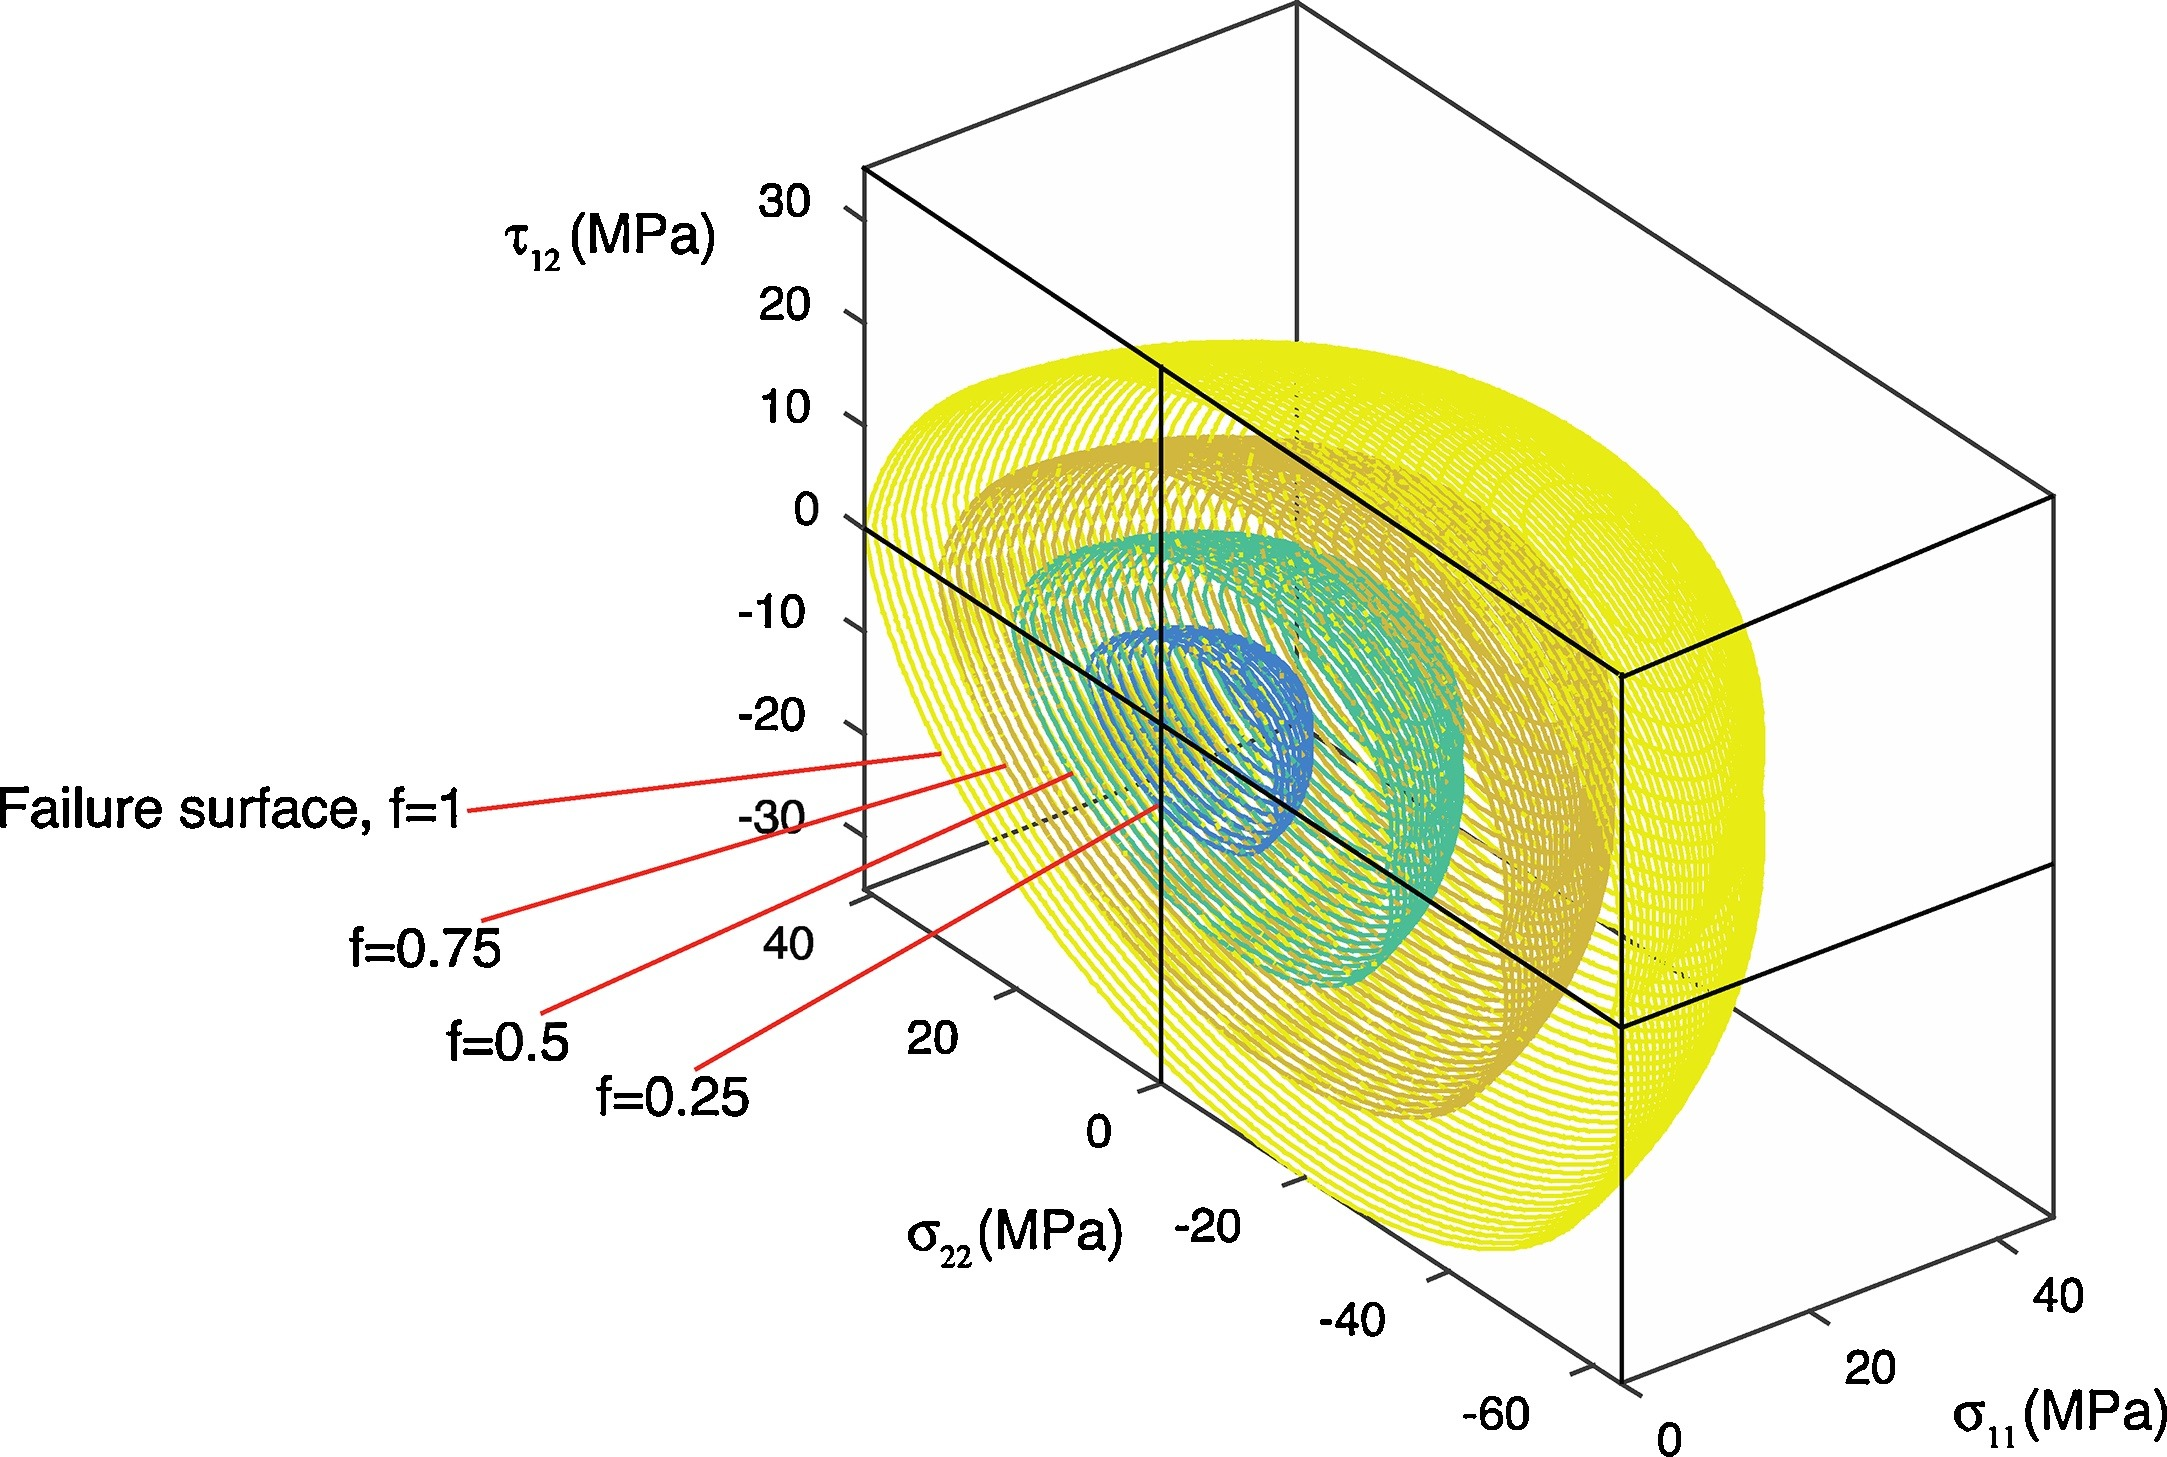
\includegraphics[height=6cm]{Obst_SLS}
	\caption{Failure surface for SLS developed through the SSIC \cite{Obst2018}} \label{fig:OOCSLS}
\end{figure}

Recent unpublished work by Osswald \emph{et al.} \cite{Osswald2020} generated a failure envelope for Multi-Jet Fusion (MJF) parts produced using PA12, and compared it to the surface obtained by Obst \emph{et al.} \cite{Obst2018}. Results indicate that, while both techniques are based on Powder Based Fusion (PBF) and use the same material, the envelopes for each AM technology were distinct, serving as proof that these technologies are not as comparable under complex loading conditions as previously assumed. The transverse-axial interaction for the MJF case was significantly less pronounced than for SLS, further reinforcing that each AM technique needs to be studied in a case-by-case basis in terms of mechanical failure characterization. 

\begin{figure}[!htbp]
	\center
	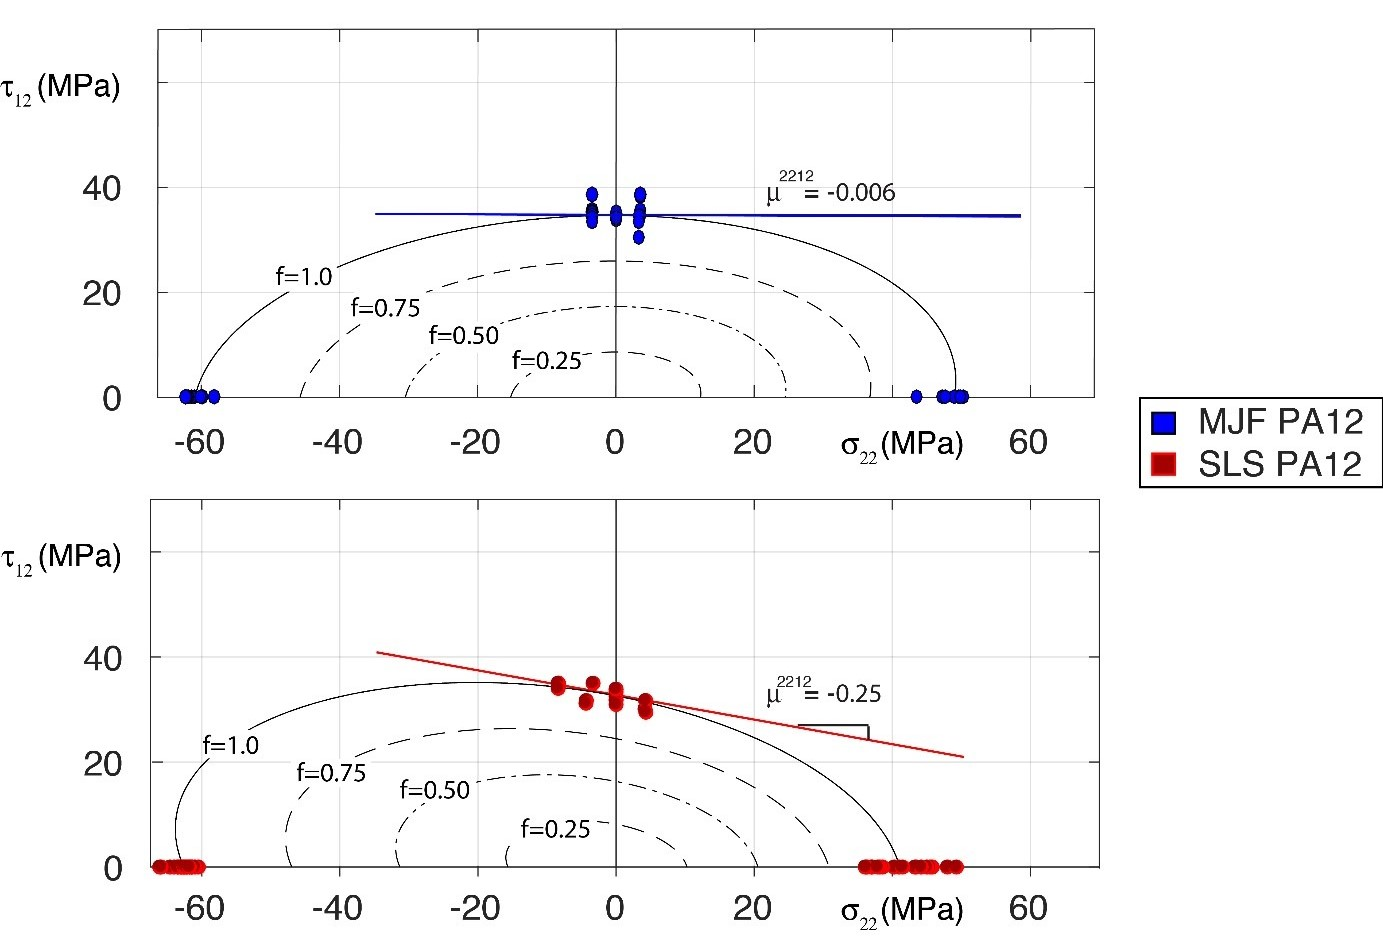
\includegraphics[height=10cm]{pbfcomp}
	\caption{Comparison of the $\sigma_{22} - \tau_{12}$ interaction for SLS and MJF PA12 parts \cite{Osswald2020}} \label{fig:pbfcomp}
\end{figure}

\section{Development of SSIC envelope for FFF parts}\label{sec:SSICFFF}

In 2019, Mazzei Capote \emph{et al.} \cite{MazzeiCapote2019} developed a failure envelope for FFF parts produced using a customized ABS filament produced in-house. Specimens were produced using either a commercially available desktop FFF printer (Lulzbot TAZ5, USA), or a customized 6-axis robotic printing solution whenever the bead orientation was hard to achieve using a \emph{2.5-D} machine. The robotic printer was based on a 6-axis robot (ABB IRB-120, Switzerland) and fitted with a stationary printhead mounted on an aluminum frame, chosen to be the same extruder from the traditional printer (LulzBot TAZ Single Extruder Tool Head v2, 0.5 mm nozzle, USA) to minimize machine influence on the results \cite{VanHulle2017}. The final surface obtained showed significant stress interactions in certain directions. Starting with the $\sigma_{11}$-$\sigma_{22}$ plane, it can be seen that the failure envelope has a slight tilt. Refer to Figure~\ref{fig:1122plane} for a graph showing the calculated failure envelope, including the experimental data for reference. This tilt is evidence of an interaction between the transverse and longitudinal stresses. The conclusion is that FFF parts produced with the print parameters used in the study should show strengthening when loaded bi-axially in compression.

\begin{figure}[h]
	\center
	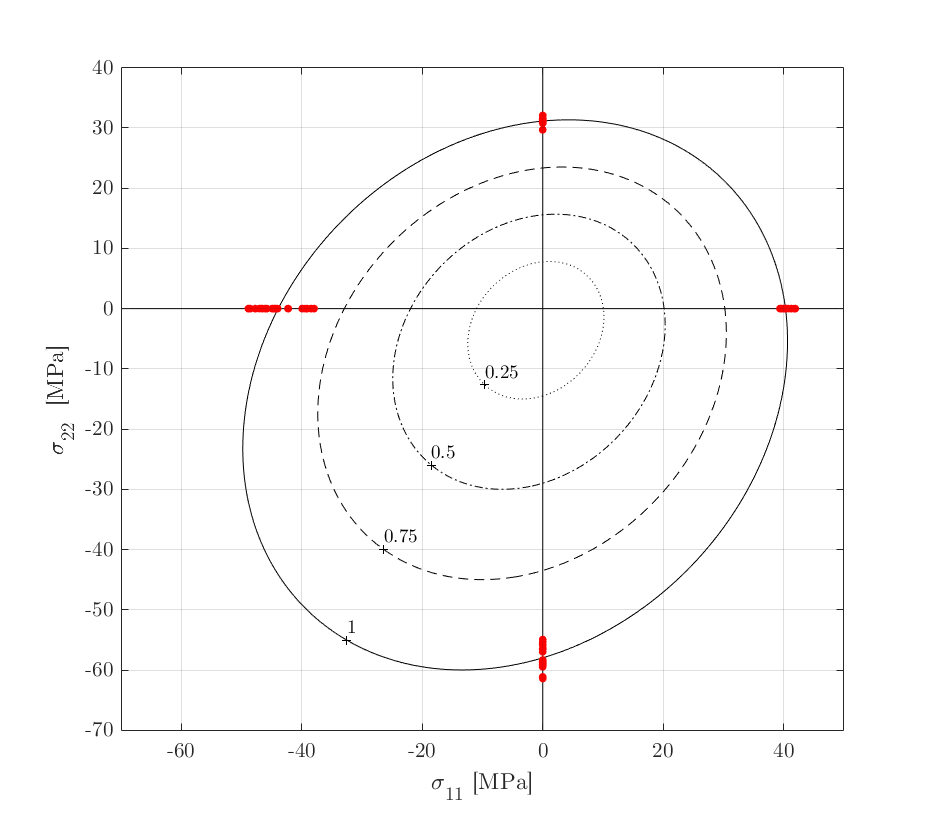
\includegraphics[width=\linewidth, keepaspectratio]{11_22plane}
	\captionsetup{justification=centering} %long caption
	\caption[failure envelope in the $\sigma_{11}$-$\sigma_{22}$ plane]{$\sigma_{11}$-$\sigma_{22}$ plane including data for reference.} \label{fig:1122plane}
\end{figure}

\pagebreak

Using the results from combined loading tests plotted in the $11-12$ and $22-12$ planes allows visualization of the transverse-axial stress interactions. Beginning with the $11-12$ plane, it can be seen that the calculated interaction slope $\mu^{1112}$ equals $5.2\times 10^{-3}$, a value that's practically zero. Using this parameter, the failure surface shown in Figure \ref{fig:1112plane} can be obtained. A dashed line representing $\mu^{1112}$ is added for reference. The $22-12$ plane by comparison reveals a considerable slope. It can be seen through the use of combined loads that there is a slight decrease in the shear strength of the specimens when a tensile load is applied in the $2-2$ direction. A slope of -0.2 was obtained for $\mu^{2212}$. Figure \ref{fig:2212plane} shows the resulting surface with the data and a line with a slope of -0.2 overlaid for reference.

\pagebreak

\begin{figure}[h]
	\center
	\subfloat[failure envelope in the $\sigma_{11}$-$\tau_{12}$ plane\label{fig:1112plane}]{%
		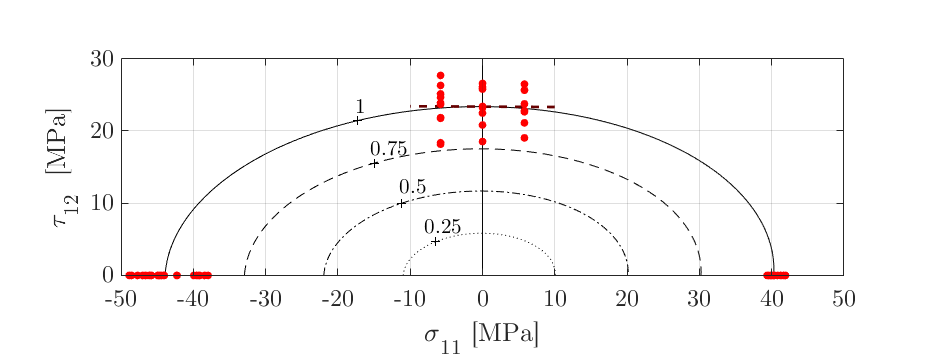
\includegraphics[width=0.9\linewidth, keepaspectratio]{11_12plane}
	}
	\linebreak
	\subfloat[failure envelope in the $\sigma_{22}$-$\tau_{12}$ plane\label{fig:2212plane}]{%
		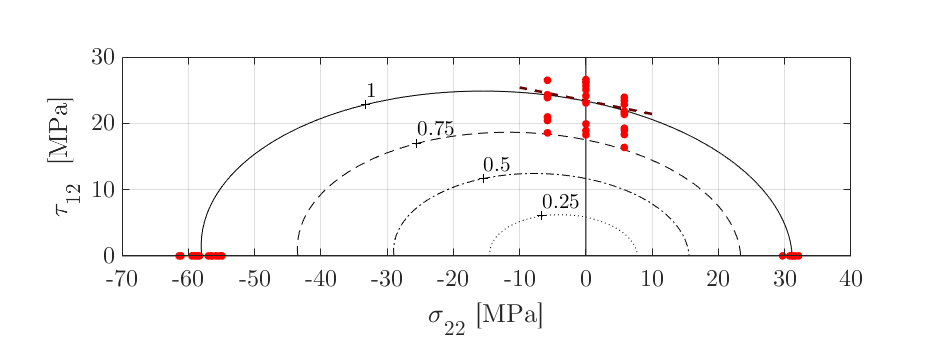
\includegraphics[width=0.9\linewidth, keepaspectratio]{22_12plane}
	}
	\caption{Comparison of interaction slopes in the axial-transverse stress planes} \label{fig:SSIcomp}
\end{figure}

\section{Validation of the FFF Failure envelope}\label{sec:FFFval}

The validity of the envelope described in Section \ref{sec:SSICFFF} was tested by Mazzei Capote  \emph{et al.} \cite{MazzeiJCompSci} in 2019. In this study, the failure function was used to estimate the failure stress of mechanical coupons loaded under tension, with a variety of raster angles being used to generate a complex loading state in the local coordinate system. Results indicated the failure prediction boundary was within 5 to 10\% of the real value. Results are summarized in Figure \ref{fig:jcompscir}, where the average of 5 mechanical tests per raster angle is represented in a dot, and the SSIC predicted failure stress is shown in a bright red line. These are compared to simpler FC, such as the maximum stress criteria in the $\sigma_{11}$, $\sigma_{22}$, and $\tau_{12}$ directions, labeled M1-1, M2-2, and M1-2 respectively. 

\begin{figure}[!htbp]
	\center
	\subfloat[Loading \label{fig:complload}]{%
		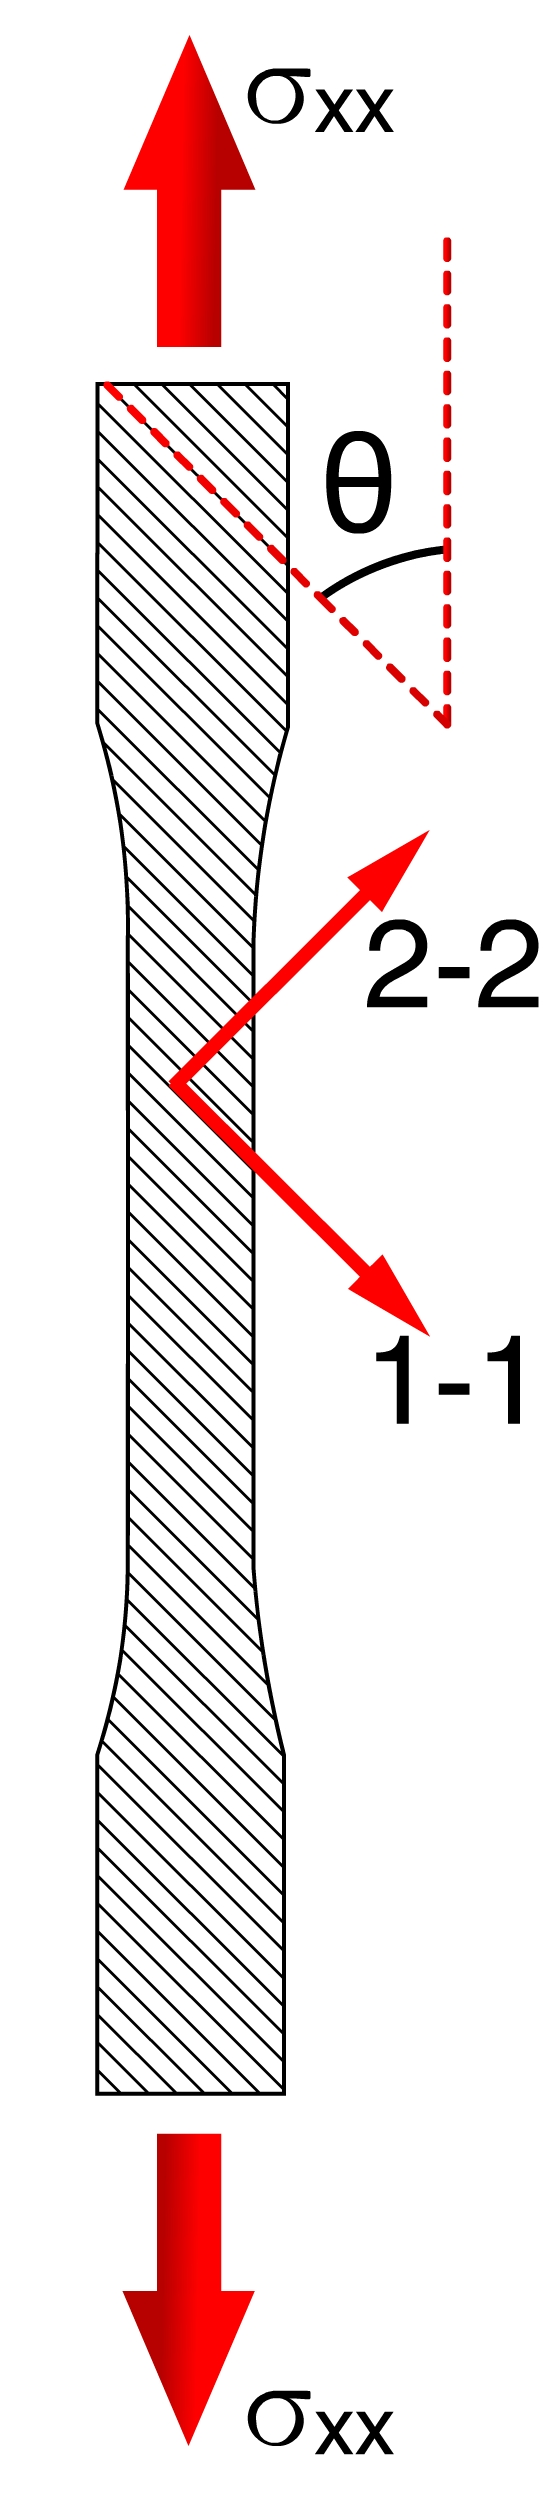
\includegraphics[height=9cm, keepaspectratio]{compl_load.jpg}
	}
	\hfill
	\subfloat[Comparison of data and failure prediction using various FC\label{fig:compsci}]{%
		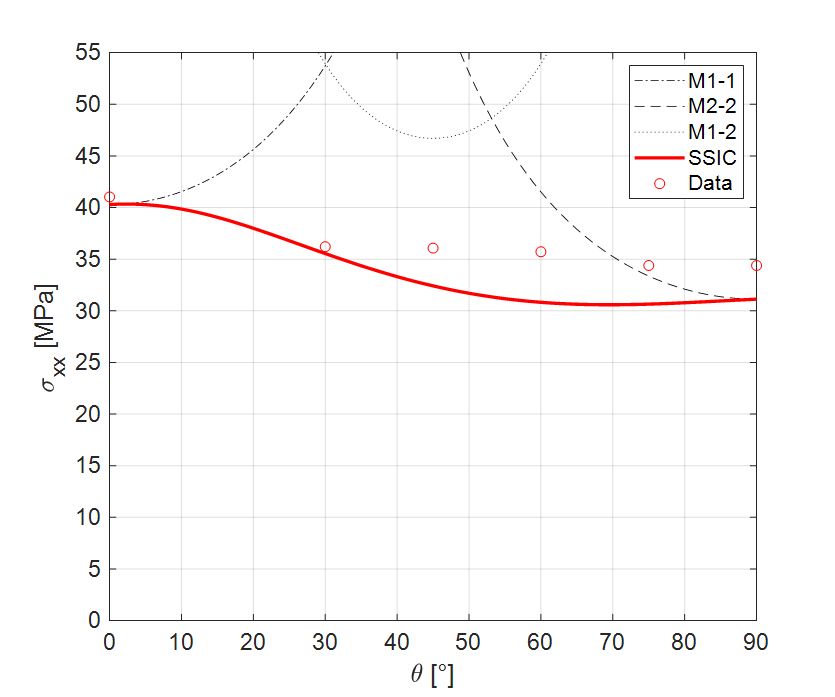
\includegraphics[height=9cm, keepaspectratio]{FC_comp.png}
	}
	\caption{Results from \cite{MazzeiJCompSci}} \label{fig:jcompscir}
\end{figure} 


While the use of FC in AM is promising, its adoption has been limited in scope. Part of the problem lies in the large number of mechanical tests required to achieve a trustworthy failure envelope, as well as the requirement of specialized equipment \textendash~such as a variety of mechanical testing devices, as well as specialized printing solutions as seen in the FFF failure envelope. Chapter \ref{ch:proposal} outlines proposed work aimed at predicting the mechanical response of FFF parts using machine learning methods. Some, if not all of the concepts explored could easily be extrapolated to other AM techniques. It should be noted that the two methods are not mutually exclusive. A combination of both FC and machine learning predictive methods can hopefully lead to a higher adoption rates of AM in industrial scenarios where the final desired application involves complex mechanical loads upon the finished part. 

% Nomenclature introduced in this chapter:
\nomenclature[A]{SSIC}{Stress-Stress Interaction Criterion}% 
\nomenclature[A]{GKC}{Gol'denblat-Kopnov Criterion}% 
\nomenclature[A]{MJF}{Multi-Jet Fusion}% 
\nomenclature[A]{PBF}{Powder Bed Fusion}% 

% Symbols introduced in this chapter:
\nomenclature[S]{$X_t$}{Tensile strength in the 1-1 direction \nomunit{$MPa$}}
\nomenclature[S]{$X_c$}{Compressive strength in the 1-1 direction \nomunit{$MPa$}}
\nomenclature[S]{$Y_t$}{Tensile strength in the 2-2 direction \nomunit{$MPa$}}
\nomenclature[S]{$Y_c$}{Compressive strength in the 2-2 direction \nomunit{$MPa$}}
\nomenclature[S]{$S$}{Shear strength in the 1-2 plane \nomunit{$MPa$}}
\nomenclature[S]{$S_{45p}$}{Positive shear strength for 45$^\circ$ specimen \nomunit{$MPa$}}
\nomenclature[S]{$S_{45n}$}{Negative shear strength for 45$^\circ$ specimen \nomunit{$MPa$}}
\nomenclature[S]{$\mu^{1112}$}{SSIC parameter- slope at pure shear failure in the $\sigma_{11}$ - $\tau_{12}$ plane \nomunit{$-$}}
\nomenclature[S]{$\mu^{2212}$}{SSIC parameter- slope at pure shear failure in the $\sigma_{22}$ - $\tau_{12}$ plane \nomunit{$-$}}
\end{document}